% File: tex/simulations.tex
% Author: Timo L. R. Halbesma <timo.halbesma@student.uva.nl>
% Version: 0.01 (Initial)
% Date created: Sat Oct 24, 2015 12:28 am
% Last modified: Mon Sep 05, 2016 01:56 AM
%
% Description: Masterthesis, Results


\documentclass[MScProj_TLRH_ClusterEnergy.tex]{subfiles}
\begin{document}
\chapter{Simulations}
\label{sec:sim}

The current \satellite{Chandra} observation constrains the emission originating 
from the baryonic content of the intra cluster medium really well. As outlined 
in chapter~\ref{sec:constrains}, this also constrains the dark matter density 
profile under the assumption of a fixed baryon fraction of 17 per cent at the 
virial radius $R_{200}$. This fully constrains both sub clusters in the Cygnus
cluster. The assumptions of hydrostatic equilibrium and spherical symmetry, 
combined with the fluid approximation allows to set up numerical representations
of both haloes using \code{Toycluster} \citep{2014MNRAS.438.1971D,
2016MNRAS.000.000D}, as outlined in chapter~\ref{sec:methods}. We assume that
the system is in a pre-merger stage around $0.2 - 0.6$ Gyr prior to core passage,
inferred by \citet{2005AJ....130...47L} from dynamical modelling the optically
visible galaxies in the Cygnus cluster. Both haloes are simulated separately
in a box with periodic boundary conditions with zero initial velocity to check
the numerical stability of the model. The single-cluster stability analysis is
presented in section~\ref{sec:SingleClusters}, followed by simulations of both
haloes in the same box in section~\ref{sec:SimulationRun}. We compare the effect
of increasing initial velocities set by a zero-energy-orbit fraction $\epsilon$.
We first consider the case where the effect of the merger shock is strongest,
which is when the merger-axis is perpendicular to the line of sight (i.e.~a 
projection angle of 90\deg). This allows us to single out the effect of increasing
the initial velocity, and therefore, the merger velocity. The results of these 
simulations are presented in section~\ref{sec:InitialVelocity}. Next, in 
section~\ref{sec:ProjectionAngle}, we take into account the effect of varying
the projection angle on the radial temperature profile for a single initial
velocity.


\section{Single Cluster Profiles and Numerical Stability}
\label{sec:SingleClusters}
We plug the following parameters into \code{Toycluster} 
(section~\ref{sec:methods-toycluster}) to generate initial conditions for one
cluster only:  i) the redshift $z=0.0562$ of Cygnus~A, ii) the total gravitating
mass $M_{200}$ enclosed in $r_{200}$, iii) the concentration parameter 
$c_{\text{NFW}}$, iv) the core radius $r_c$, and v) the betamodel slope $b$.
The numerical values are given in Table~\ref{tab:parameters} in 
section~\ref{sec:gas-to-dm}. The mass ratio is set to zero and we generate initial
conditions such that each sub cluster individually is placed in a box with periodic
boundary conditions. The code uses the B-Spline kernel with $50 \pm 0.05$ neighbours
in the SPH smoothing length search, and relaxes the clusters using Weighted Voronoi 
Tesselations. The resulting sampled numerical density profiles are shown in 
Figure~\ref{fig:cygA_stability_ic} and Figure~\ref{fig:cygB_stability_ic} for CygA,
respectively CygB. The observed density profiles are overplotted to check that the
sampled haloes indeed match the observations presented in 
section~\ref{sec:numberdensity} and section~\ref{sec:results-xray}. 

Next, we feed the initial conditions file to \code{Gadget-2} to integrate both 
haloes over $5$~Gyr to check how well the density profile remains over a timescale 
significantly longer than the expected time before the merger takes, should both 
clusters be placed in the same box on a collision course. The single-cluster
stability check is presented in Figure~\ref{fig:cygA_stability_011} for CygA,
respectively Figure~\ref{fig:cygB_stability_011} for CygB. Trough out the simulations,
both haloes do show a slight increase in the density profile in the central region. 
This behaviour was hypothesised to result from changing the kernel when going
from \code{Toycluster} to \code{Gadget-2}. However, both codes now use the same
kernel and the same number of neighbours to smooth over. Therefore we consider
it unlikely that the density increase within the kernel is purely a result of
feeding to the particles to the second stage in the simulation pipeline. The
second noticeable change that the sampled profiles beyond $2 r_{200}$ no longer
exactly follow the analytical model after $5$~Gyr. At these radii the halo feels
a nearby cluster (itself) as the box has periodic boundary conditions. The models
are not valid in this boundary region, thus, this region is shaded out by the
grey rectangle. The central density strongly influences the observed X-ray
surface brightness, which could prove troublesome later on as the CygB halo
shows a significant temperature increase and the sampled halo does not match very
well with the observation. Overall, the clusters do seem stable over a long
integration timescale and we consider it save to use this setup to simulate the 
merger in the following section.

\clearpage
\begin{figure}
    \centering
    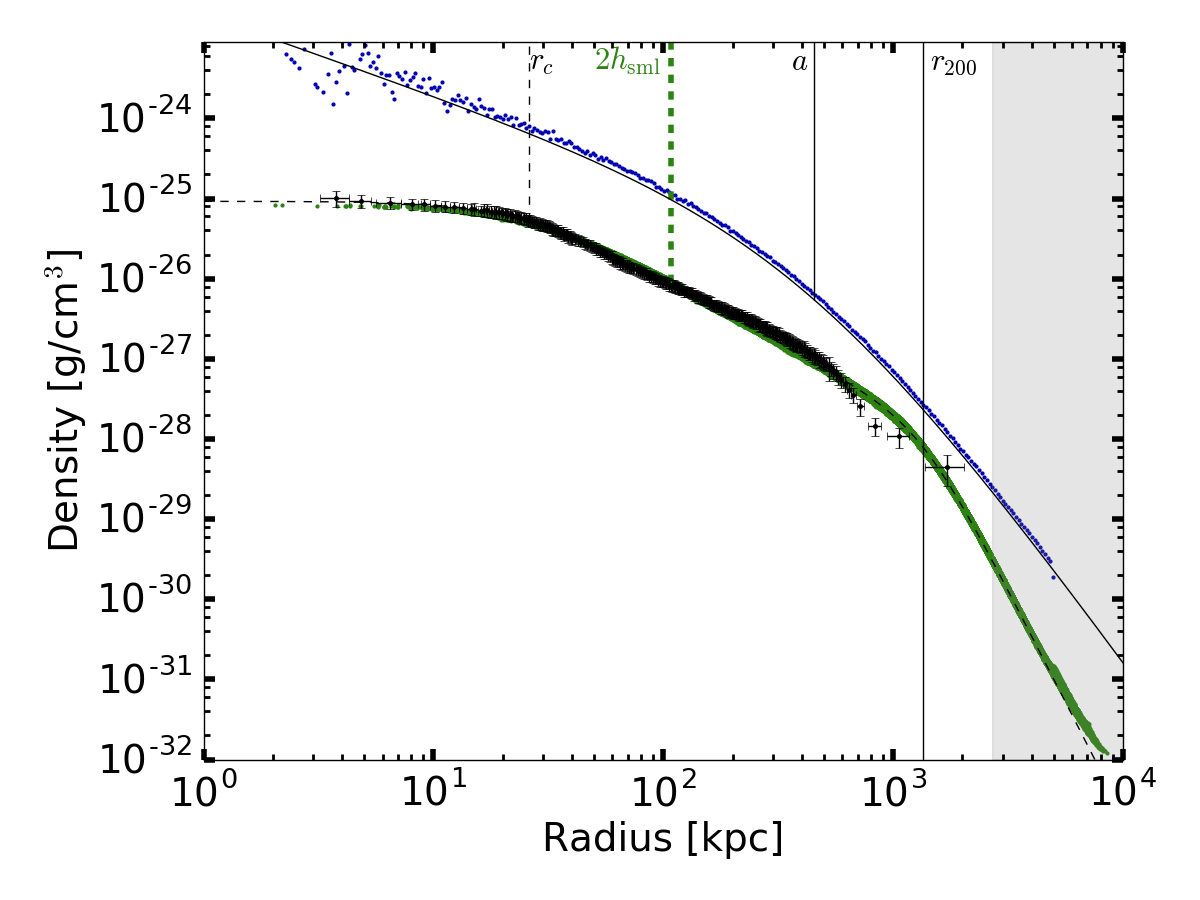
\includegraphics[width=0.9\textwidth]{sim/stability/cygA_stability_ic.png}
    \caption{Radial density profile of CygA produced by \code{Toyclyster} using
             two million particles. The numerically sampled initial conditions
             have a gas profile (green) that matches nicely with the observations
             (black dots with errorbars), both overplotted on the analytical model
             (dashed). The vertical green dashed line shows the resolution scale,
             the core radius $r_c$, the Hernquist scale length $a$ and the viral
             radius $r_{200}$ are also indicated with vertical lines. The shaded
             grey area indicates the boundary region where the model is not valid.}
    \label{fig:cygA_stability_ic}
    \centering
    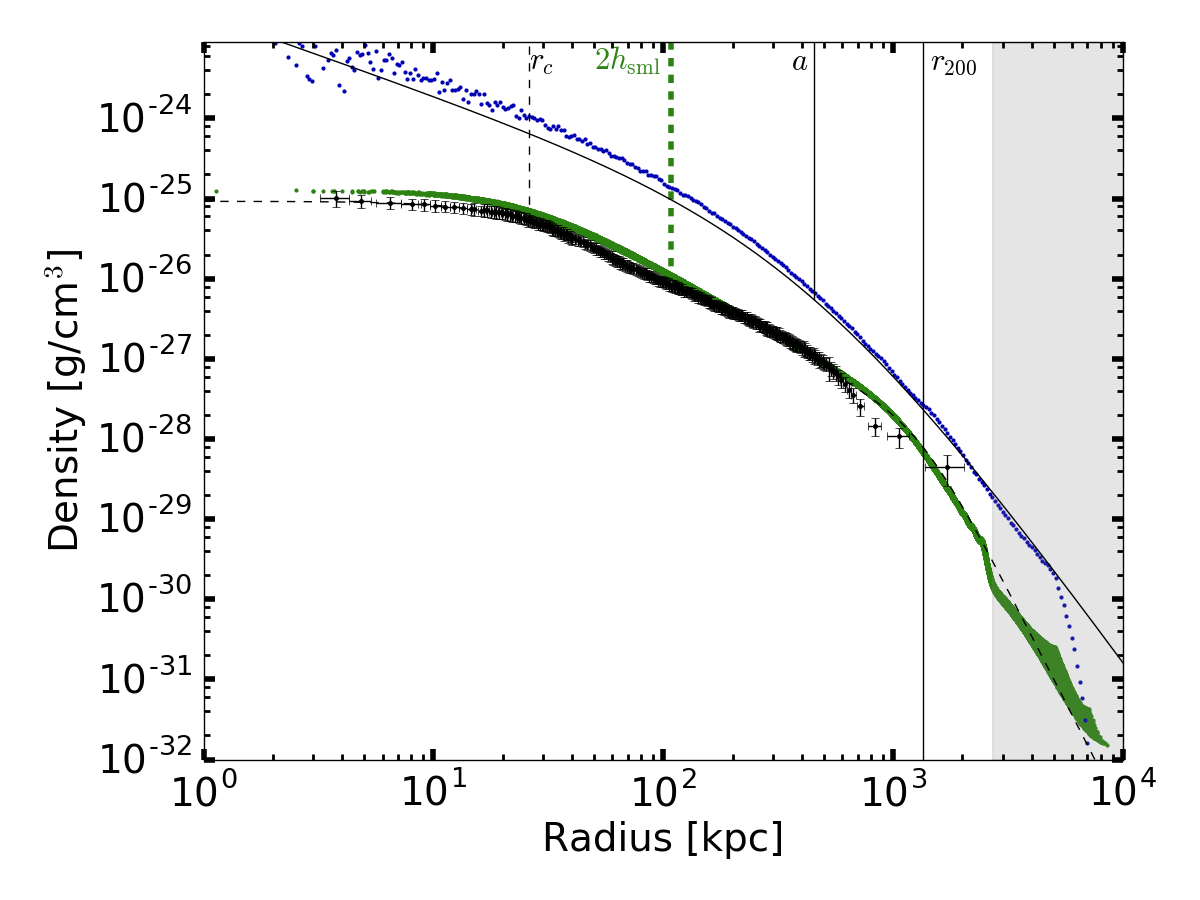
\includegraphics[width=0.9\textwidth]{sim/stability/cygA_stability_011.png}
    \caption{Same plot of CygA after integrating for $5$~Gyr with \code{Gadget-2}.}
    \label{fig:cygA_stability_011}
\end{figure}
\clearpage
\begin{figure}
    \centering
    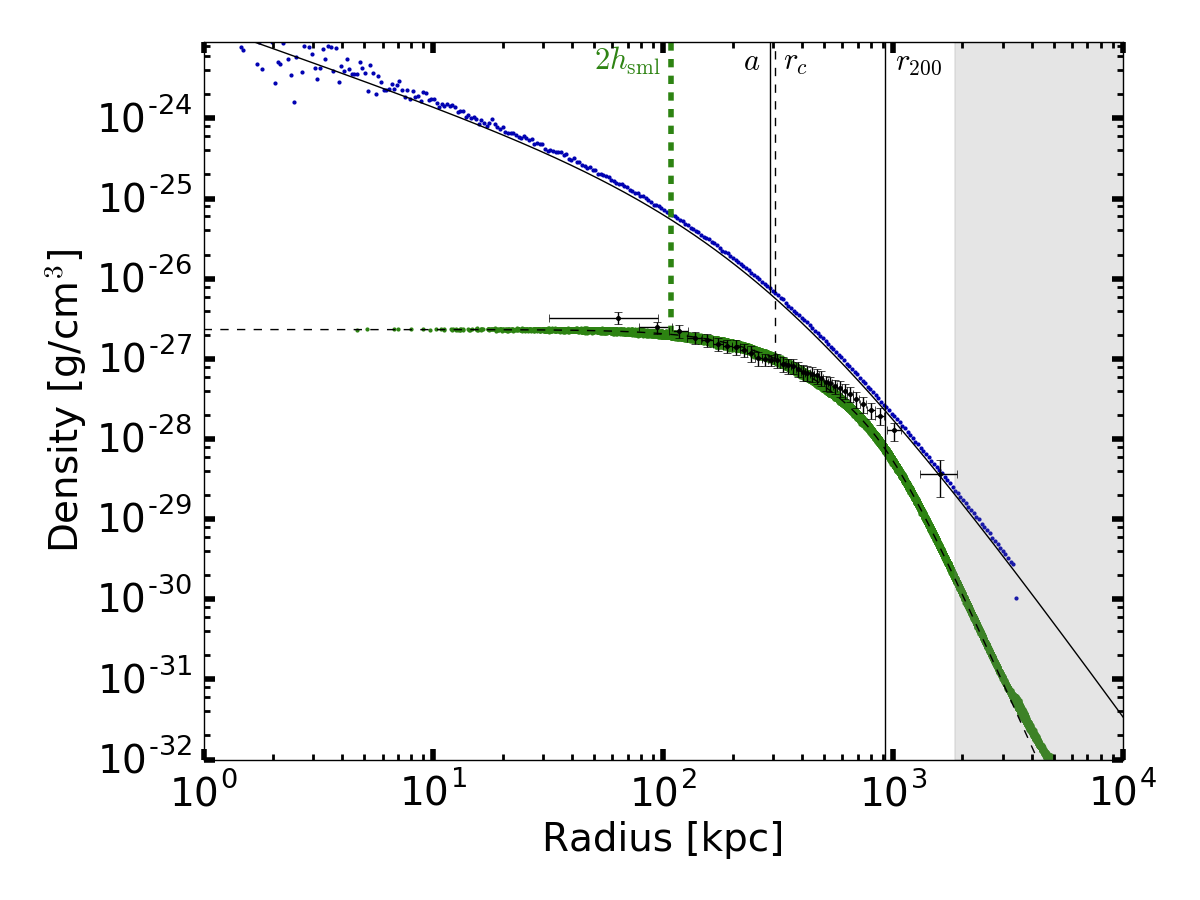
\includegraphics[width=0.9\textwidth]{sim/stability/cygB_stability_ic.png}
    \caption{Radial density profile of CygB produced by \code{Toyclyster} using
             two million particles. The numerically sampled initial conditions
             have a gas profile (green) that matches acceptably with the observations
             (black dots with errorbars), both overplotted on the analytical model
             (dashed). The vertical green dashed line shows the resolution scale,
             the core radius $r_c$, the Hernquist scale length $a$ and the viral
             radius $r_{200}$ are also indicated with vertical lines. The shaded
             grey area indicates the boundary region where the model is not valid.}
    \label{fig:cygB_stability_ic}
    \centering
    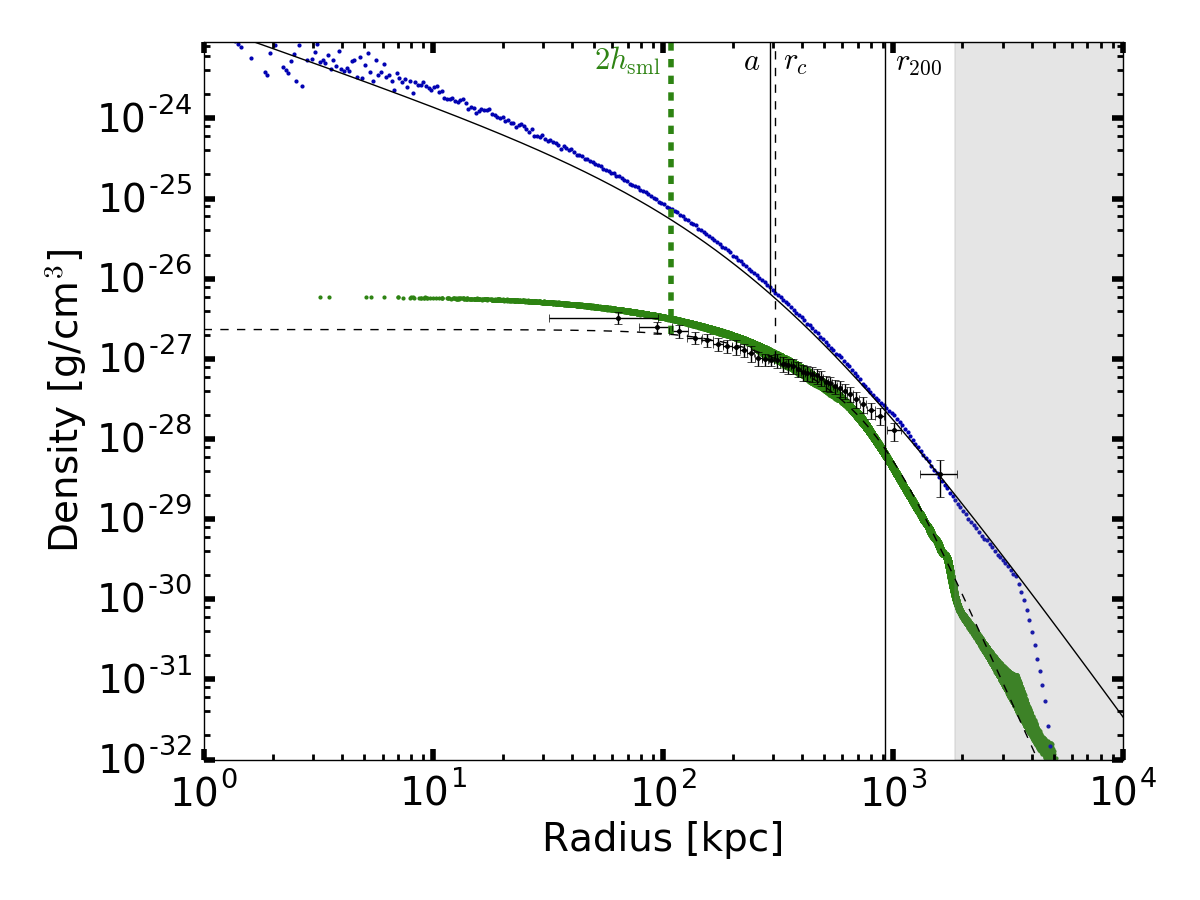
\includegraphics[width=0.9\textwidth]{sim/stability/cygB_stability_011.png}
    \caption{Same plot of CygB after integrating for $5$~Gyr with \code{Gadget-2}.}
    \label{fig:cygB_stability_011}
\end{figure}


\clearpage
\section{Simulation Runs with Stable Clusters}
\label{sec:SimulationRun}
As a first check we show that the numerical radial density profiles match the
\satellite{Chandra} observation presented in chapter~\ref{sec:constrains}.
Figure~\ref{fig:cygA_stability_ic} and Figure~\ref{fig:cygB_stability_ic} clearly
show that this is the case, although these figures are obtained when the clusters
were sampled individually in a box. Moreover, the first snapshot written by 
\code{Gadget-2} starts with the particle properties of the initial conditions created
by \code{Toycluster}, but the hydrodynamic quantities are immediately recalculated. 
Therefore we explicitly check that the content of this file indeed represents
the observed clusters. The radial density profile of snapshots that contain two
haloes can be created by making a histogram of the dark matter density along the 
merger axis, which shows two peaks. The cluster centroids can then found at the
pixel-value of highest density, while the minimum between the peaks shows how
far the clusters had to be shifted to make their virial radii touch. The box can
then split up between particles where x-positions above and below the minimum-density
position belong to the cluster on the right (CygB), respectively the halo on the
left-hand side of the box (CygA). The radii can be calculated with respect to their
shifted origin, and the radial density profile can then be plotted. As of yet, 
the implementation of this halo-finding algorithm requires improvement. On the
other hand, \code{Toycluster} gives the position of the centroid, which is used
to shift back the haloes, calculate the radii, plot the radial density profile.
However, naturally this only works for the zeroth snapshot which is before the 
clusters are displaced. The resulting plots (not included) are very comparable
to the single-cluster stability plots, although quite a lot of particles are 
assigned to the wrong cluster and the profiles look more messy for that reason.

We now turn to the third simulation step, and consider the extreme case that the 
merger-axis is perpendicular to the line of sight such that we can run the 
line-of-sight integration and projection code \code{P-Smac2} 
\citep{2014MNRAS.443.3564D}, as presented in section~\ref{sec:methods-psmac}.
The expected temperature jump will be the largest when the merger is viewed edge-on. 
Other projection angles will lower the temperature with an angle-dependent 
constant factor. We use \code{P-Smac2} to generate fits cubes of the projected 
X-ray surface brightness and spectroscopic temperature. The second comparison
of the simulated results is with the observed \satellite{Chandra} X-ray surface 
brightness, Figure~\ref{fig:CygA_Xray_extended} in section~\ref{sec:xray}. 
Several snapshots taken at different times are placed around the observation 
in Figure~\ref{fig:snapz}. The values do not match quantitatively as no
unit conversions were done yet, but seen comparable qualitatively.
To check if the numbers also match, the next challenge is to find 
out which snapshot best-represents the cluster environment of Cygnus~A. 
Figure~\ref{fig:ruler} in section~\ref{sec:xray} shows the \satellite{Chandra} 
observation where a ruler overplotted to measure the projected core separation. 
The distance found is $700.621''$, thus, the simulation snapshot chosen is such
that the simulated distance between CygA and CygB is $700$ kpc. The distance is
approximated by swapping seconds of arc for kpc as $1'' \approx 1$~kpc at the 
redshift of the system when using generic cosmological parameters. The 
simulations provide the size of the entire simulated box in kpc, and a number of 
pixels can be specified at runtime for \code{P-Smac2}. This allows to calculate 
the pixelscale, and the distance in physical unit is found by multiplying the 
number of pixels between the cluster centroids by the pixelscale. 


\begin{figure}
    \makebox[\textwidth][c]{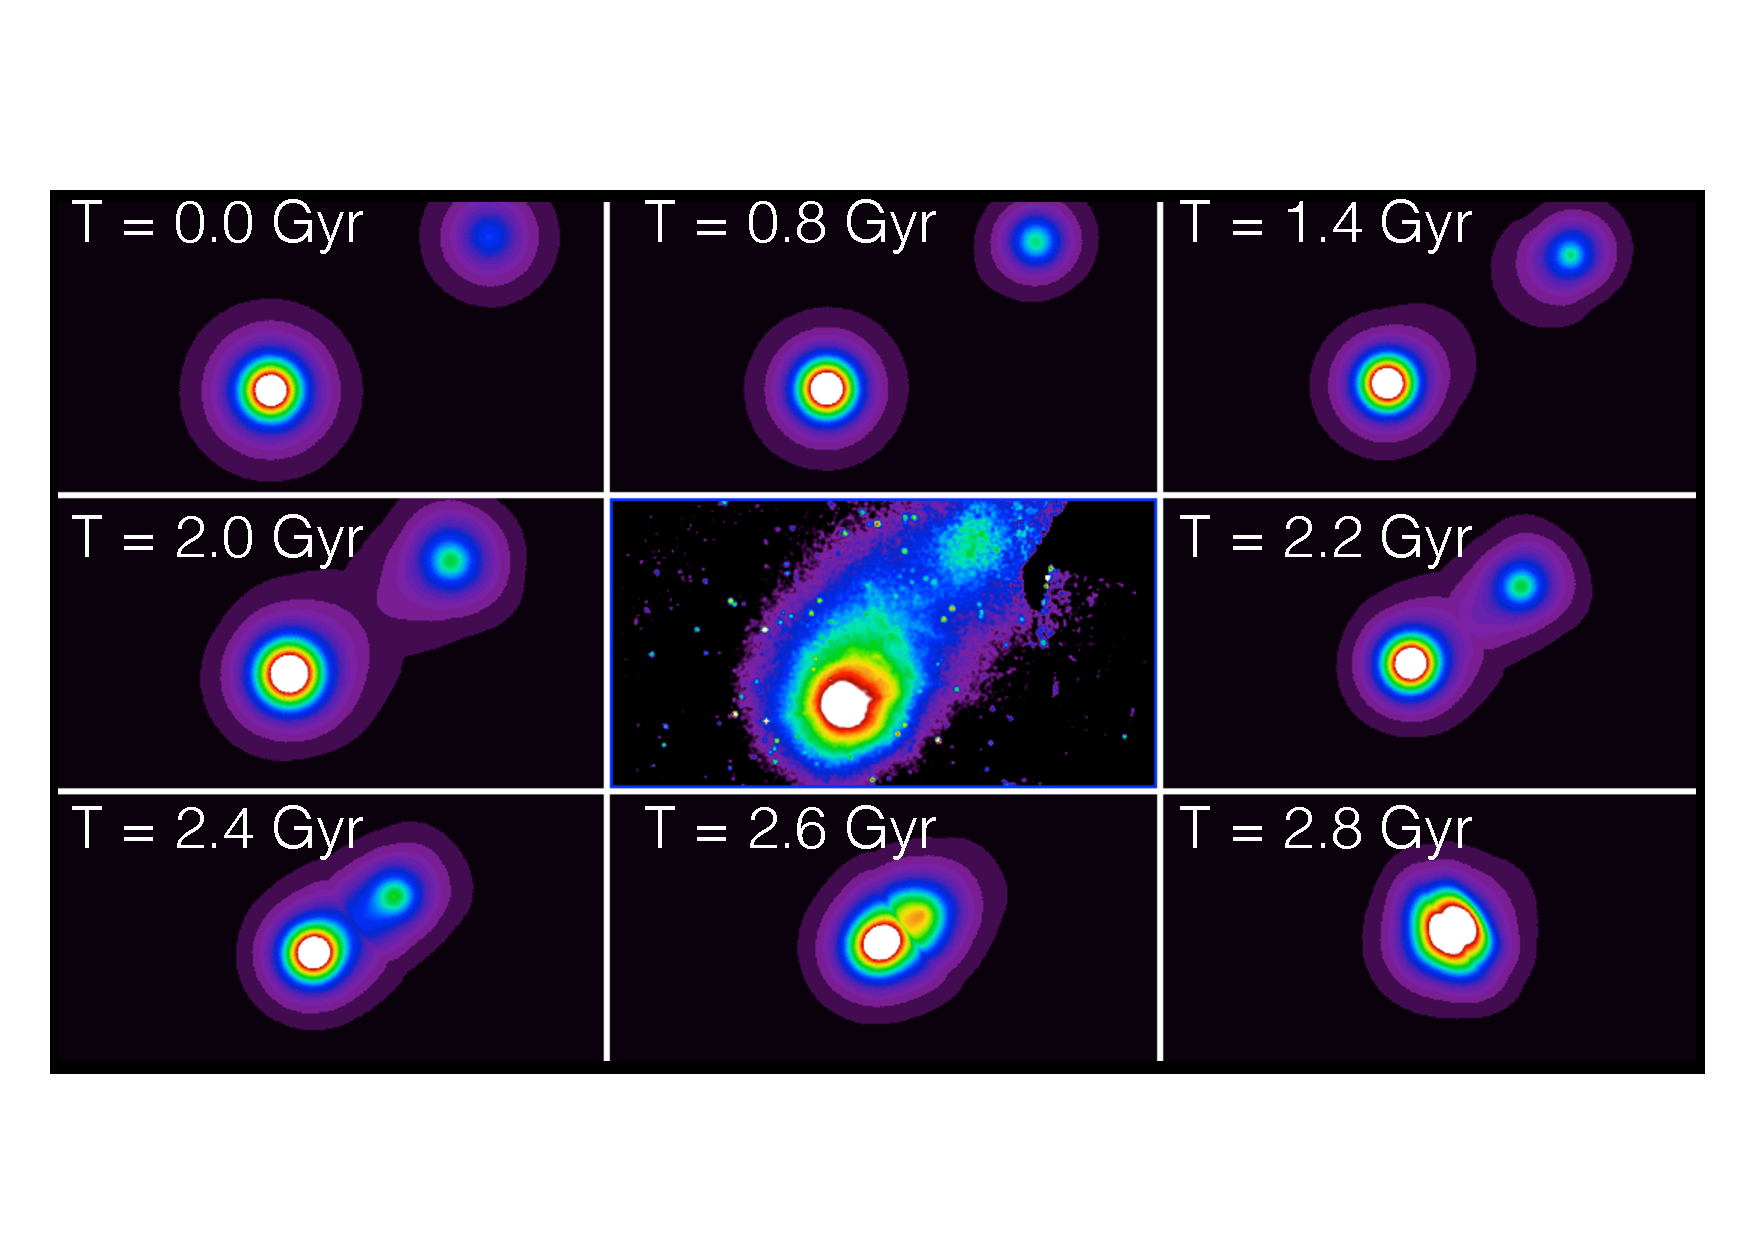
\includegraphics[width=1.3\textwidth]{sim/snapshot_xray.pdf}}%
    \caption{Projected 90\deg \, X-ray surface brightness of the simulations
             surrounding the \satellite{Chandra} observation.}
    \label{fig:snapz}
\end{figure}

% Attempt to get radial density profile. Problem: P-Smac2 gives 2D projected 
% gas density in g/cm^2. How do I obtain radial number density in 1/cm^3?
%The radial density profile is created by taking the \code{P-Smac2} 
%\citep{2014MNRAS.443.3564D} physical density output. The numerical setup is shown
%in Figure~\ref{fig:VirialRadiiTouch} first snapshot
%\begin{figure}
%\centering
%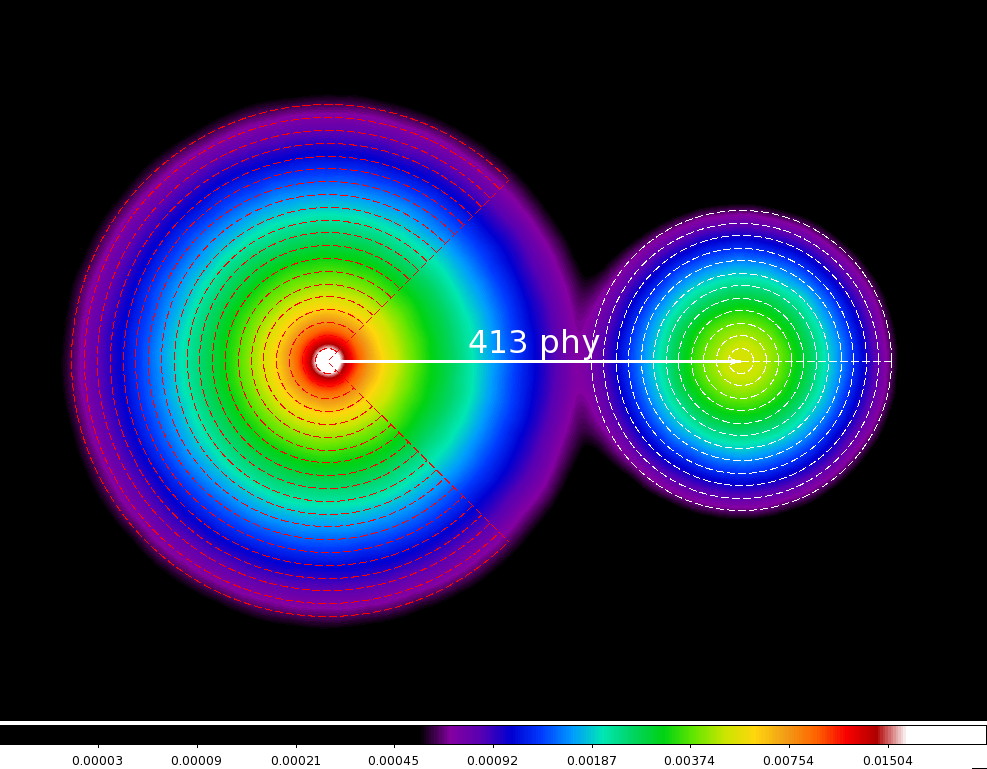
\includegraphics[width=0.75\textwidth]{sim/density/20160820T0403_1_TouchingVirialRadiiPlusDensityExtractionRegion.png}
%\caption{figure}
%\label{fig:VirialRadiiTouch}
%\end{figure}







\newpage
\subsection{Varying the initial velocity}
\label{sec:InitialVelocity}
Now that we know which snapshot is appropriate to select, three different models
are used where the merger velocity is varied. The maximum initial velocity is 
reached when all available gravitational energy is converted to kinetic
energy. \code{Toycluster} sets the velocities of both haloes as follows, and the 
difference is called the initial velocity.

\begin{align}
    v_{\text{CygA}} &= \epsilon  \sqrt{2G ( M_{\text{CygA}} +  M_{\text{CygA}})/d}
     \label{eq:zeroeorbitfrac} \\
    v_{\text{CygB}} &= - \frac{ M_{200}}{M_{\text{CygB}}} \cdot v_{\text{CygA}} 
     \quad ,
\end{align}

\noindent where $M_{\text{CygA}}$ and $M_{\text{CygB}}$ are the final sampled 
masses while $M_{200}$ is value of the desired total gravitating mass given as an
input parameter to \code{Toycluster}. The constant $\epsilon$ is the zero-energy orbit
fraction, where $\epsilon = 0$ is the unlikely situation that the infilling cluster
starts at a distance $d = \infty$. Furthermore, values larger than unity are
unphysical as more gravitational energy would be required than available in the 
system. As time progresses in the simulations, the velocity further increases.
The final velocity difference between both clusters at the snapshot chosen is 
referred to as the merger velocity. The quantitative values are estimated from a
histogram of the gas velocity in the $x$-direction (along the merger-axis).
Figure~\ref{fig:VelocityDetermination} shows both the clean initial velocities,
and the rather messy merger velocity distribution of the gas in the $x$-direction.
The latter shows a broad spread, so the merger velocity is a rough estimate with 
a best-guess error margin of $\pm$ 200 km/s. We expect the particles in the region
between both sub clusters to have the highest velocities, so the largest possible 
velocity difference is quoted. Table~\ref{tab:VelocityGrid} shows an overview of
three $\epsilon$-values chosen to investigate the effect that the merger velocity
has on the expected merger-induced temperature jump. Simulations are distinguishable
by a timestamp. 

\begin{table}
    \centering
    \caption{Simulations with increasing velocities}
    \label{tab:VelocityGrid}
    \begin{tabular}{lcccc}
        \hline
        SimulationID & $\epsilon$ & $v_{\text{initial}}$ (km/s) & Snapshot & $v_{\text{merger}}$ (km/s) \\
        \hline
        20160819T2322 & $0.0$ & $0$ & $91$ & \mytilde $1400$ \\
        %20160819T2357 & $0.1$ & $159$ & $77$ & \mytilde $1400$ \\
        %20160820T0032 & $0.2$ & $318$ & $68$ & \mytilde $1600$ \\
        20160820T0107 & $0.3$ & $474$ & $60$ & \mytilde $1700$ \\
        %20160820T0142 & $0.4$ & $635$ & $53$ & \mytilde $1650$ \\
        %20160820T0218 & $0.5$ & $795$ & $47$ & \mytilde $1700$ \\
        %20160820T0252 & $0.6$ & $954$ & $43$ & \mytilde $1900$ \\
        %20160820T0328 & $0.7$ & $1113$ & $39$ & \mytilde $1950$ \\
        20160820T0403 & $0.8$ & $1271$ & $35$ & \mytilde $2050$ \\
        %20160820T0438 & $0.9$ & $1430$ & $33$ & \mytilde $2200$ \\
        %20160820T0513 & $1.0$ & $1589$ & & \\
        \hline
    \end{tabular}
\end{table}

\begin{figure}
    \centering
    \begin{subfigure}{.5\textwidth}
        \centering
        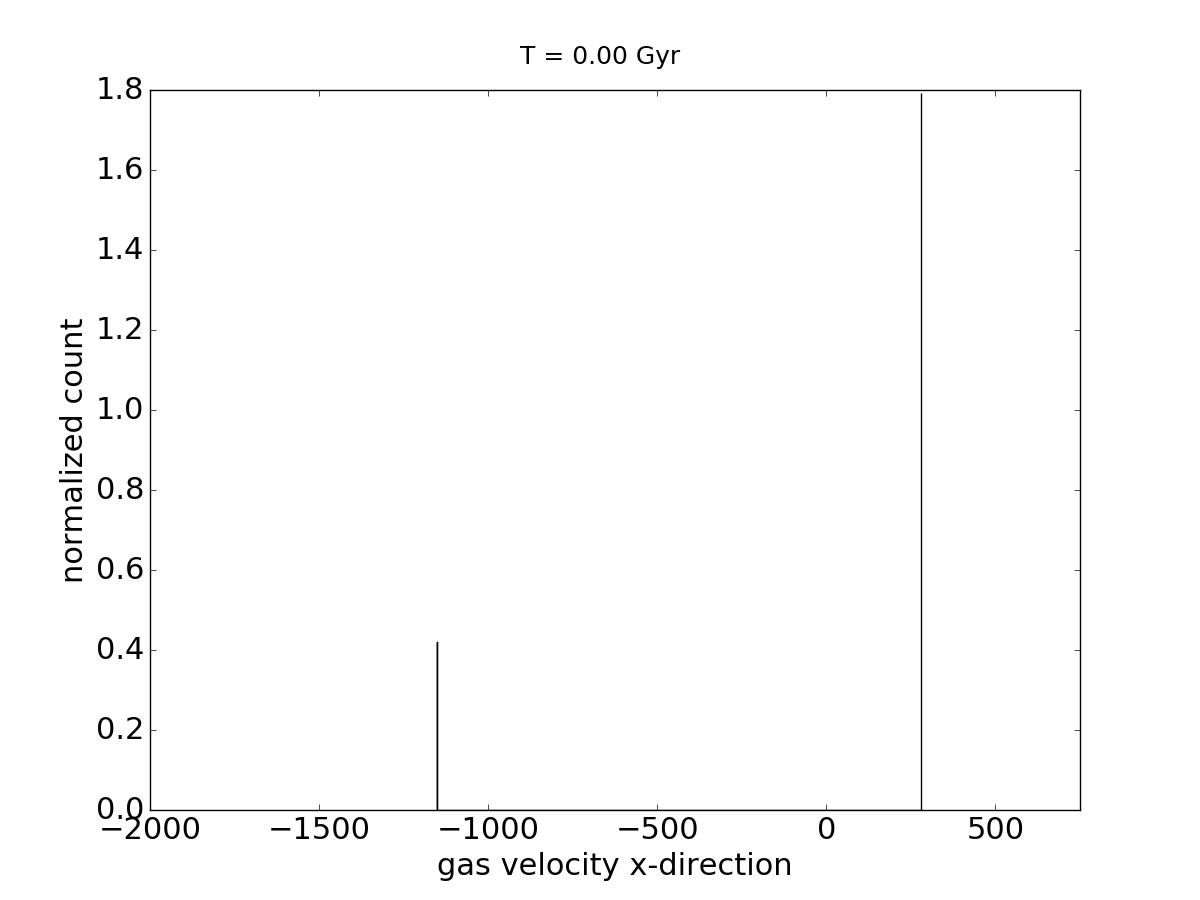
\includegraphics[width=\linewidth]{sim/vel/20160820T0438_gasvx_000.png}
    \end{subfigure}%
    \begin{subfigure}{.5\textwidth}
        \centering
        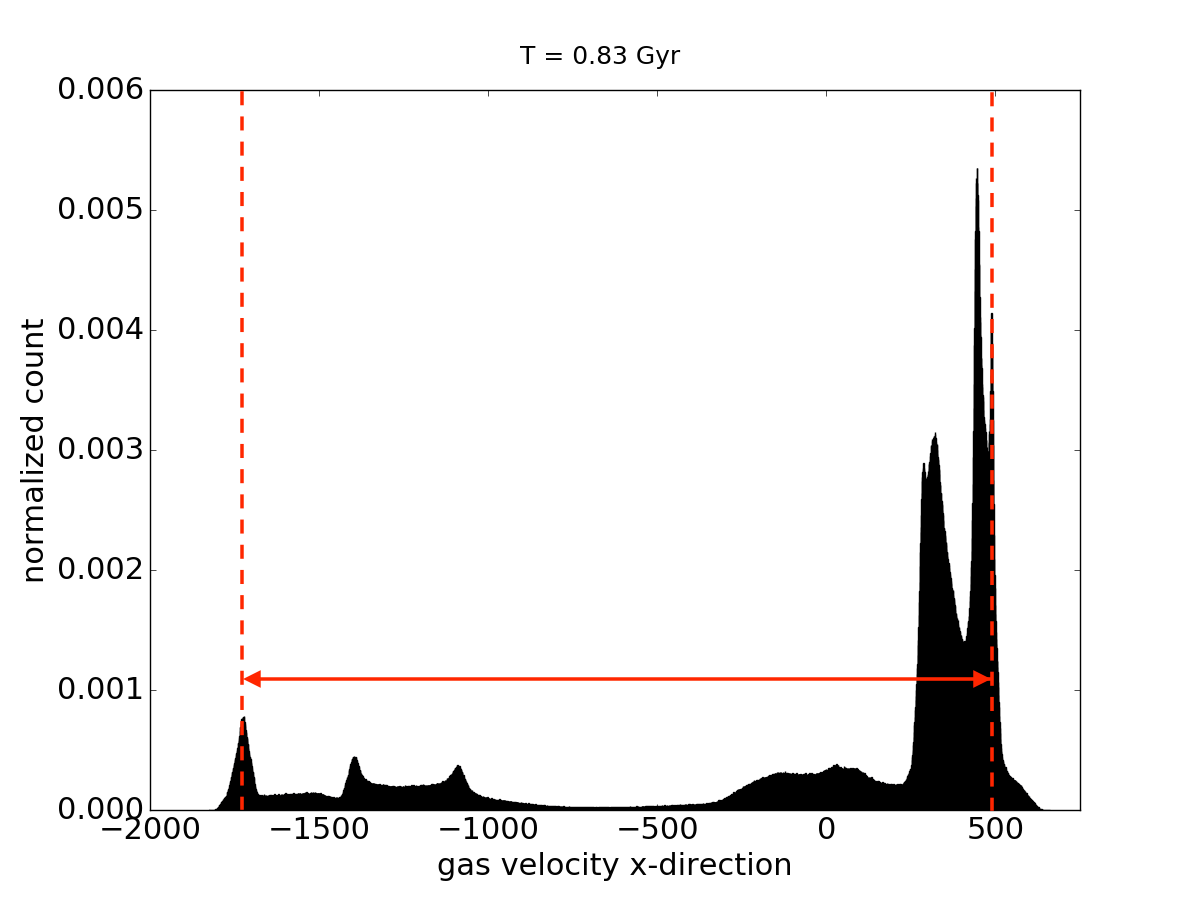
\includegraphics[width=\linewidth]{sim/vel/20160820T0438_gasvx_033.png}
    \end{subfigure}
    \caption{Gas velocity in the $x$-direction. 
             Left: initial velocity $v_{\text{initial}}$. 
             Right: merger velocity $v_{\text{merger}}$.}
    \label{fig:VelocityDetermination}
\end{figure}

The simulated temperature profiles can be extracted from the given snapshot using 
SAOImage~ds9 \citep{2003ASPC..295..489J}. However, the documentation is rather
unclear what the program does exactly under the hood. Therefore a self-written 
\code{Python} script is used as well. The effect of the merger is excluded by
cutting out a 90\deg \, wedge centered on the simulated model that represents
CygA. The same method that was used in section~\ref{sec:numberdensity} and 
section~\ref{sec:ChandraTemperature} is followed to create a 'quiescent' 
temperature profile as well as a 'merger' temperature profile. Within ds9, using
\mybox{Region} $\rightarrow$ \mybox{Shape} $\rightarrow$ \mybox{Panda} allows the
user to create a wedge centered on given $x, y$ pixel values, spanning a given
total range of radii placed at a given number of intervals, while using a given
upper and lower angle and the number of wedges placed inbetween. Then, in the 
panda menu, selecting \mybox{Analysis} $\rightarrow$ \mybox{Radial Profile} creates
the desired radial profile taken within the wedge at the desired radii, which can
be saved to a data file. Both the average and the merger wedges are centered on 
the simulated representation of the Cygnus~A cluster. The merger-axis is horizontal 
given the projection used, so the merger-wedge starts at $-45^\circ$ and ends at 
$45^\circ$, where the zero angle is defined as the horizontal line from the center
to the maximum radius. This either extracts the mean, median, average or perhaps
uses some other way to determine the values but the exact method was not found
in the documentation. For this reason the temperature profiles are extracted
using a \code{Python} script that does the aforementioned and takes the median
values. The extraction regions are presented in Figure~\ref{fig:20160819T2322_E},
where the red lines overplotted on the spectroscopic temperature show the average
region while the white lines indicate the merger-wedge. Within the wedges the
number of spherical shells is $42$, starting at $r=0$ up to a radius of $r=200$ 
pixels. This gives the `raw' radial temperature profiles. The pixels on the x-axis 
are then converted from physical units (pixels) to kpc. The size of the entire box
is $10105$ kpc, and the fits-files have a total of $2048$ pixels in the $x$ and in
the $y$ direction, which gives a conversion factor of $10105/2048\approx 4.93$ kpc 
per pixel. The temperature on the y-axis is converted from Kelvin to keV by 
multiplying by the Boltzmann constant $kB = 8.62 \cdot 10^{-8}$~keV/K. The resulting 
simulated temperature structure is shown in Figure~\ref{fig:20160819T2322_T}
together with the average and merger \satellite{Chandra} profiles. The simulation
appears to show a temperature structure that appears $1.5$~keV cooler than
observed

Furthermore, a \satellite{Suzaku} observation of Cygnus~A is also shown in the
same plot. These data are reproduced (by eye) from \citet{2013AN....334..346S},
and the x-axis is converted from arcminutes to kpc.

\clearpage
\begin{figure}
    \centering
    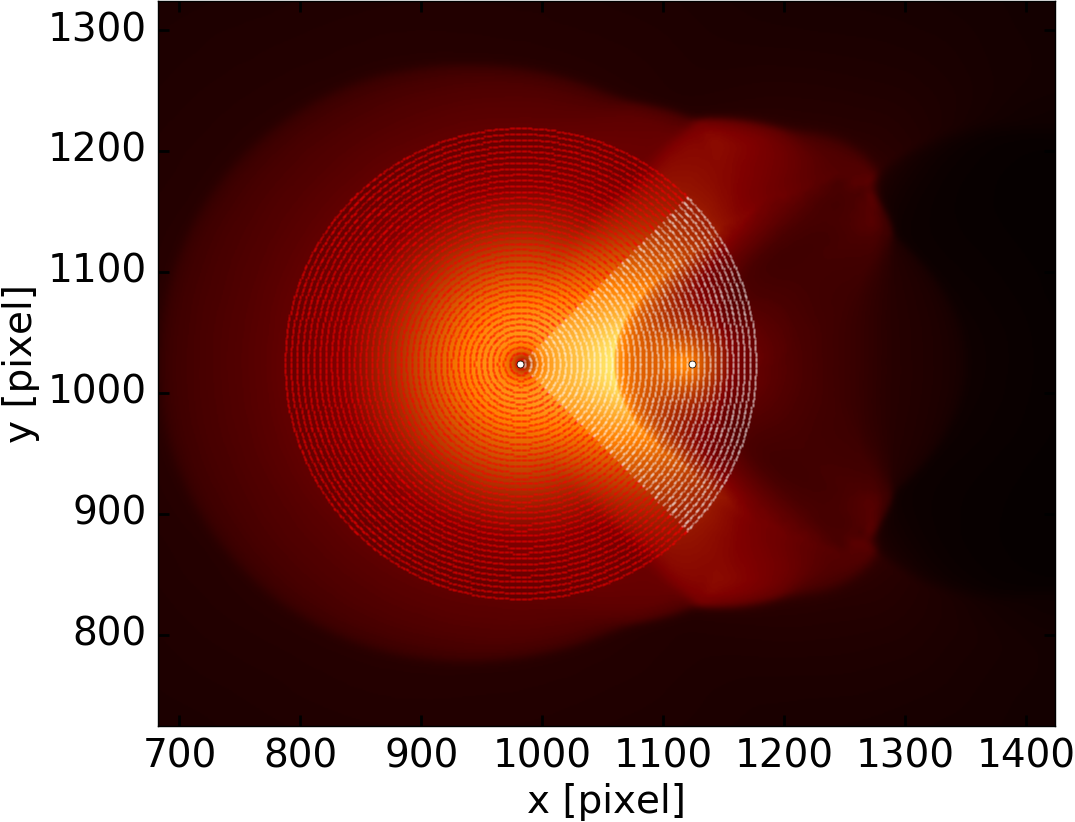
\includegraphics[width=0.85\textwidth]{sim/temperature/20160819T2322_extraction.png}
    \caption{Spherical wedges used to extract the simulated radial temperature 
             profile from the line-of-sight integrated spectroscopic temperature 
             output of \code{P-Smac2} in the $\epsilon = 0.0$ simulation. The red 
             shells indicate the extraction region 
             of the average profile, while the white wedge shows the merger-axis.
             The total boxsize in this snapshot is $10105$~kpc for $2048^2$ pixels,
             so the pixelscale is $4.93$. The distance between the two white dots
             indicating the centroids is roughly $142$~pixels, or $700$~kpc.}
    \label{fig:20160819T2322_E}
    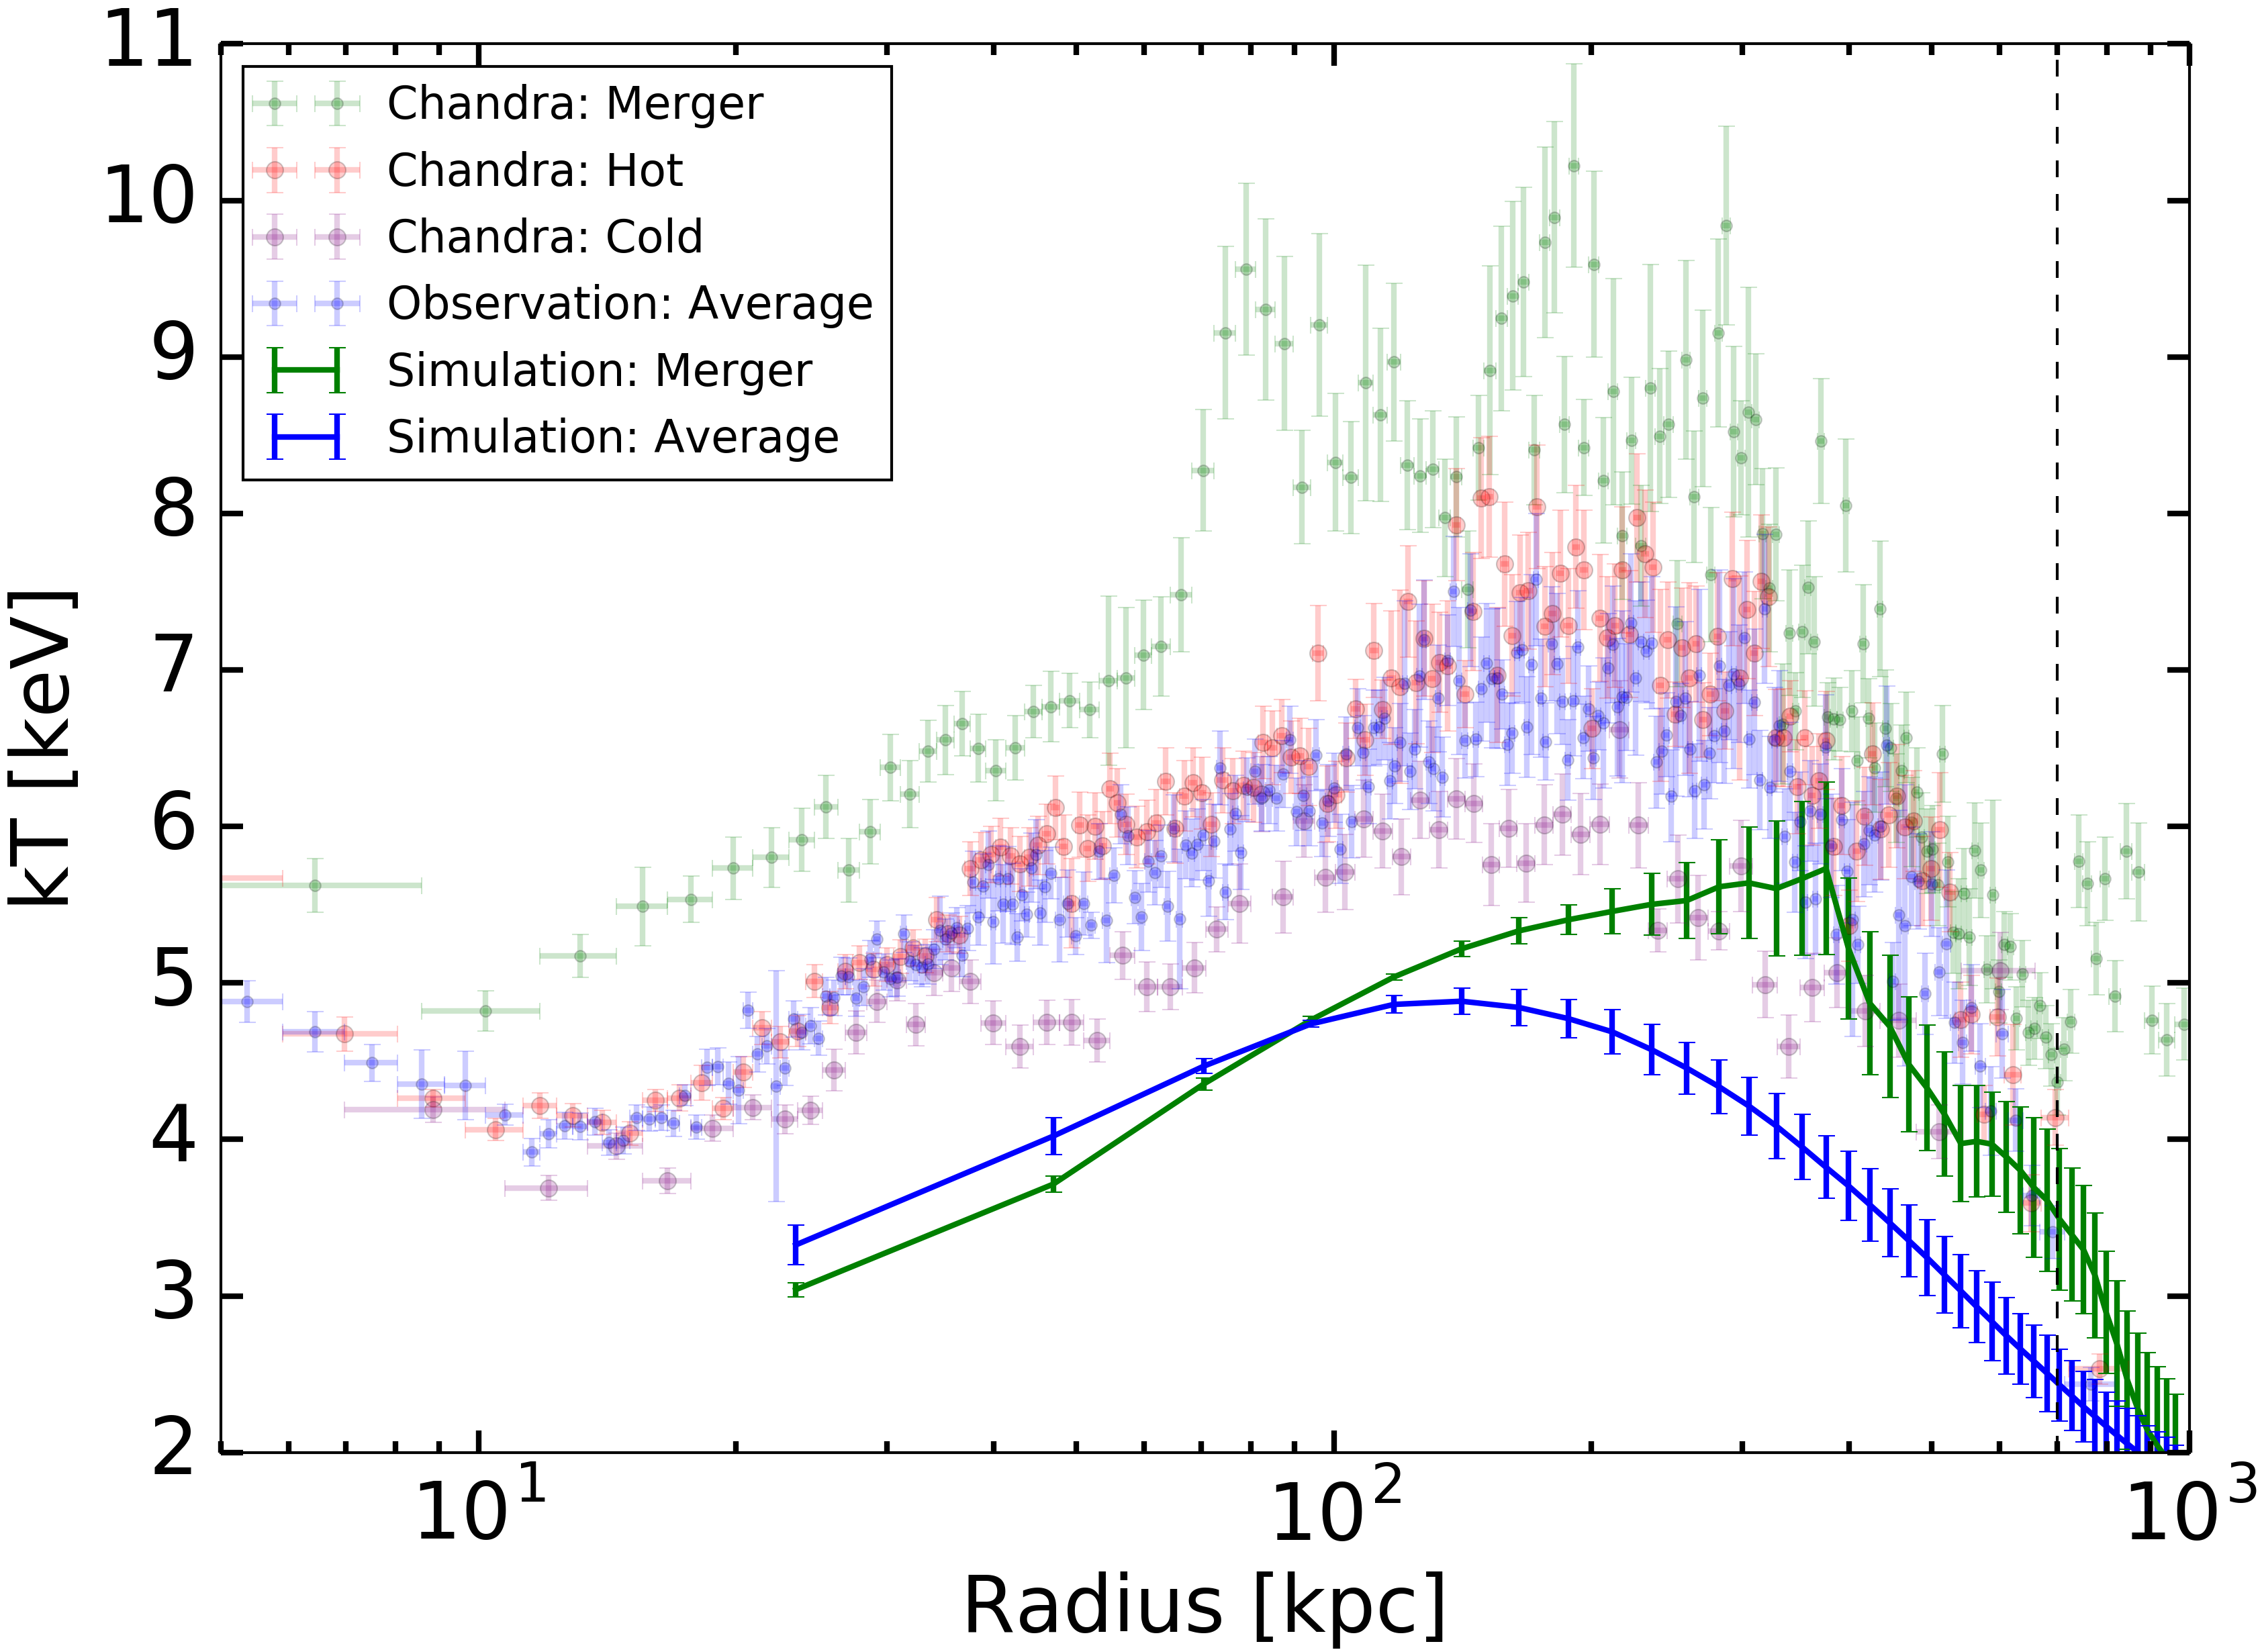
\includegraphics[width=0.85\textwidth]{sim/temperature/20160819T2322_temperature.png}
    \caption{Simulated radial temperature profiles after converting units of the raw 
             profiles to temperature in keV versus distance along the merger axis in
             kpc. The data points show the temperature structure observed by 
             \satellite{Chandra}. The green points show the merger wedge, while the 
             blue markers indicate the average profile. The simulated temperature 
             appears to be $1.5$~keV lower than observed.}
    \label{fig:20160819T2322_T}
\end{figure}
\clearpage
\begin{figure}
    \centering
    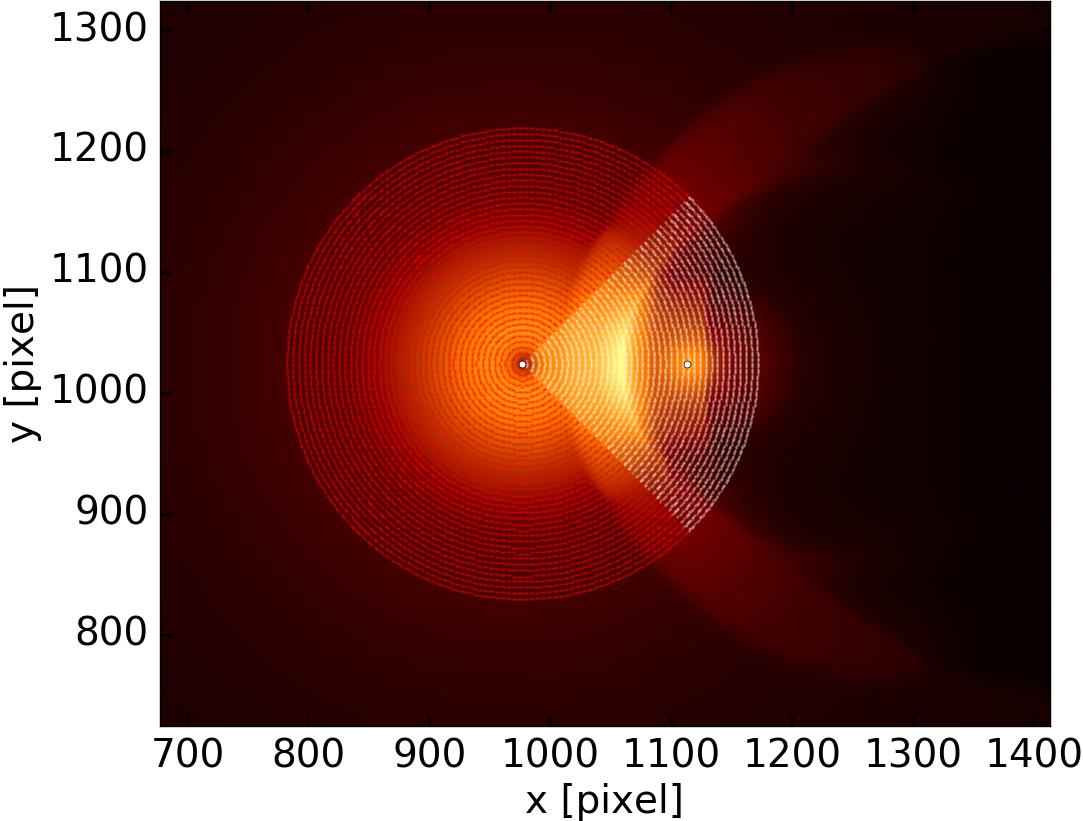
\includegraphics[width=0.85\textwidth]{sim/temperature/20160820T0403_extraction.png}
    \caption{Extraction regions of the $\epsilon = 0.8$ simulation. The 
             parabolic orbit can clearly be seen here, but the merger temperature
             appears to be insensitive to the initial (and merger) velocity.}
    \label{fig:20160820T0403_E}
    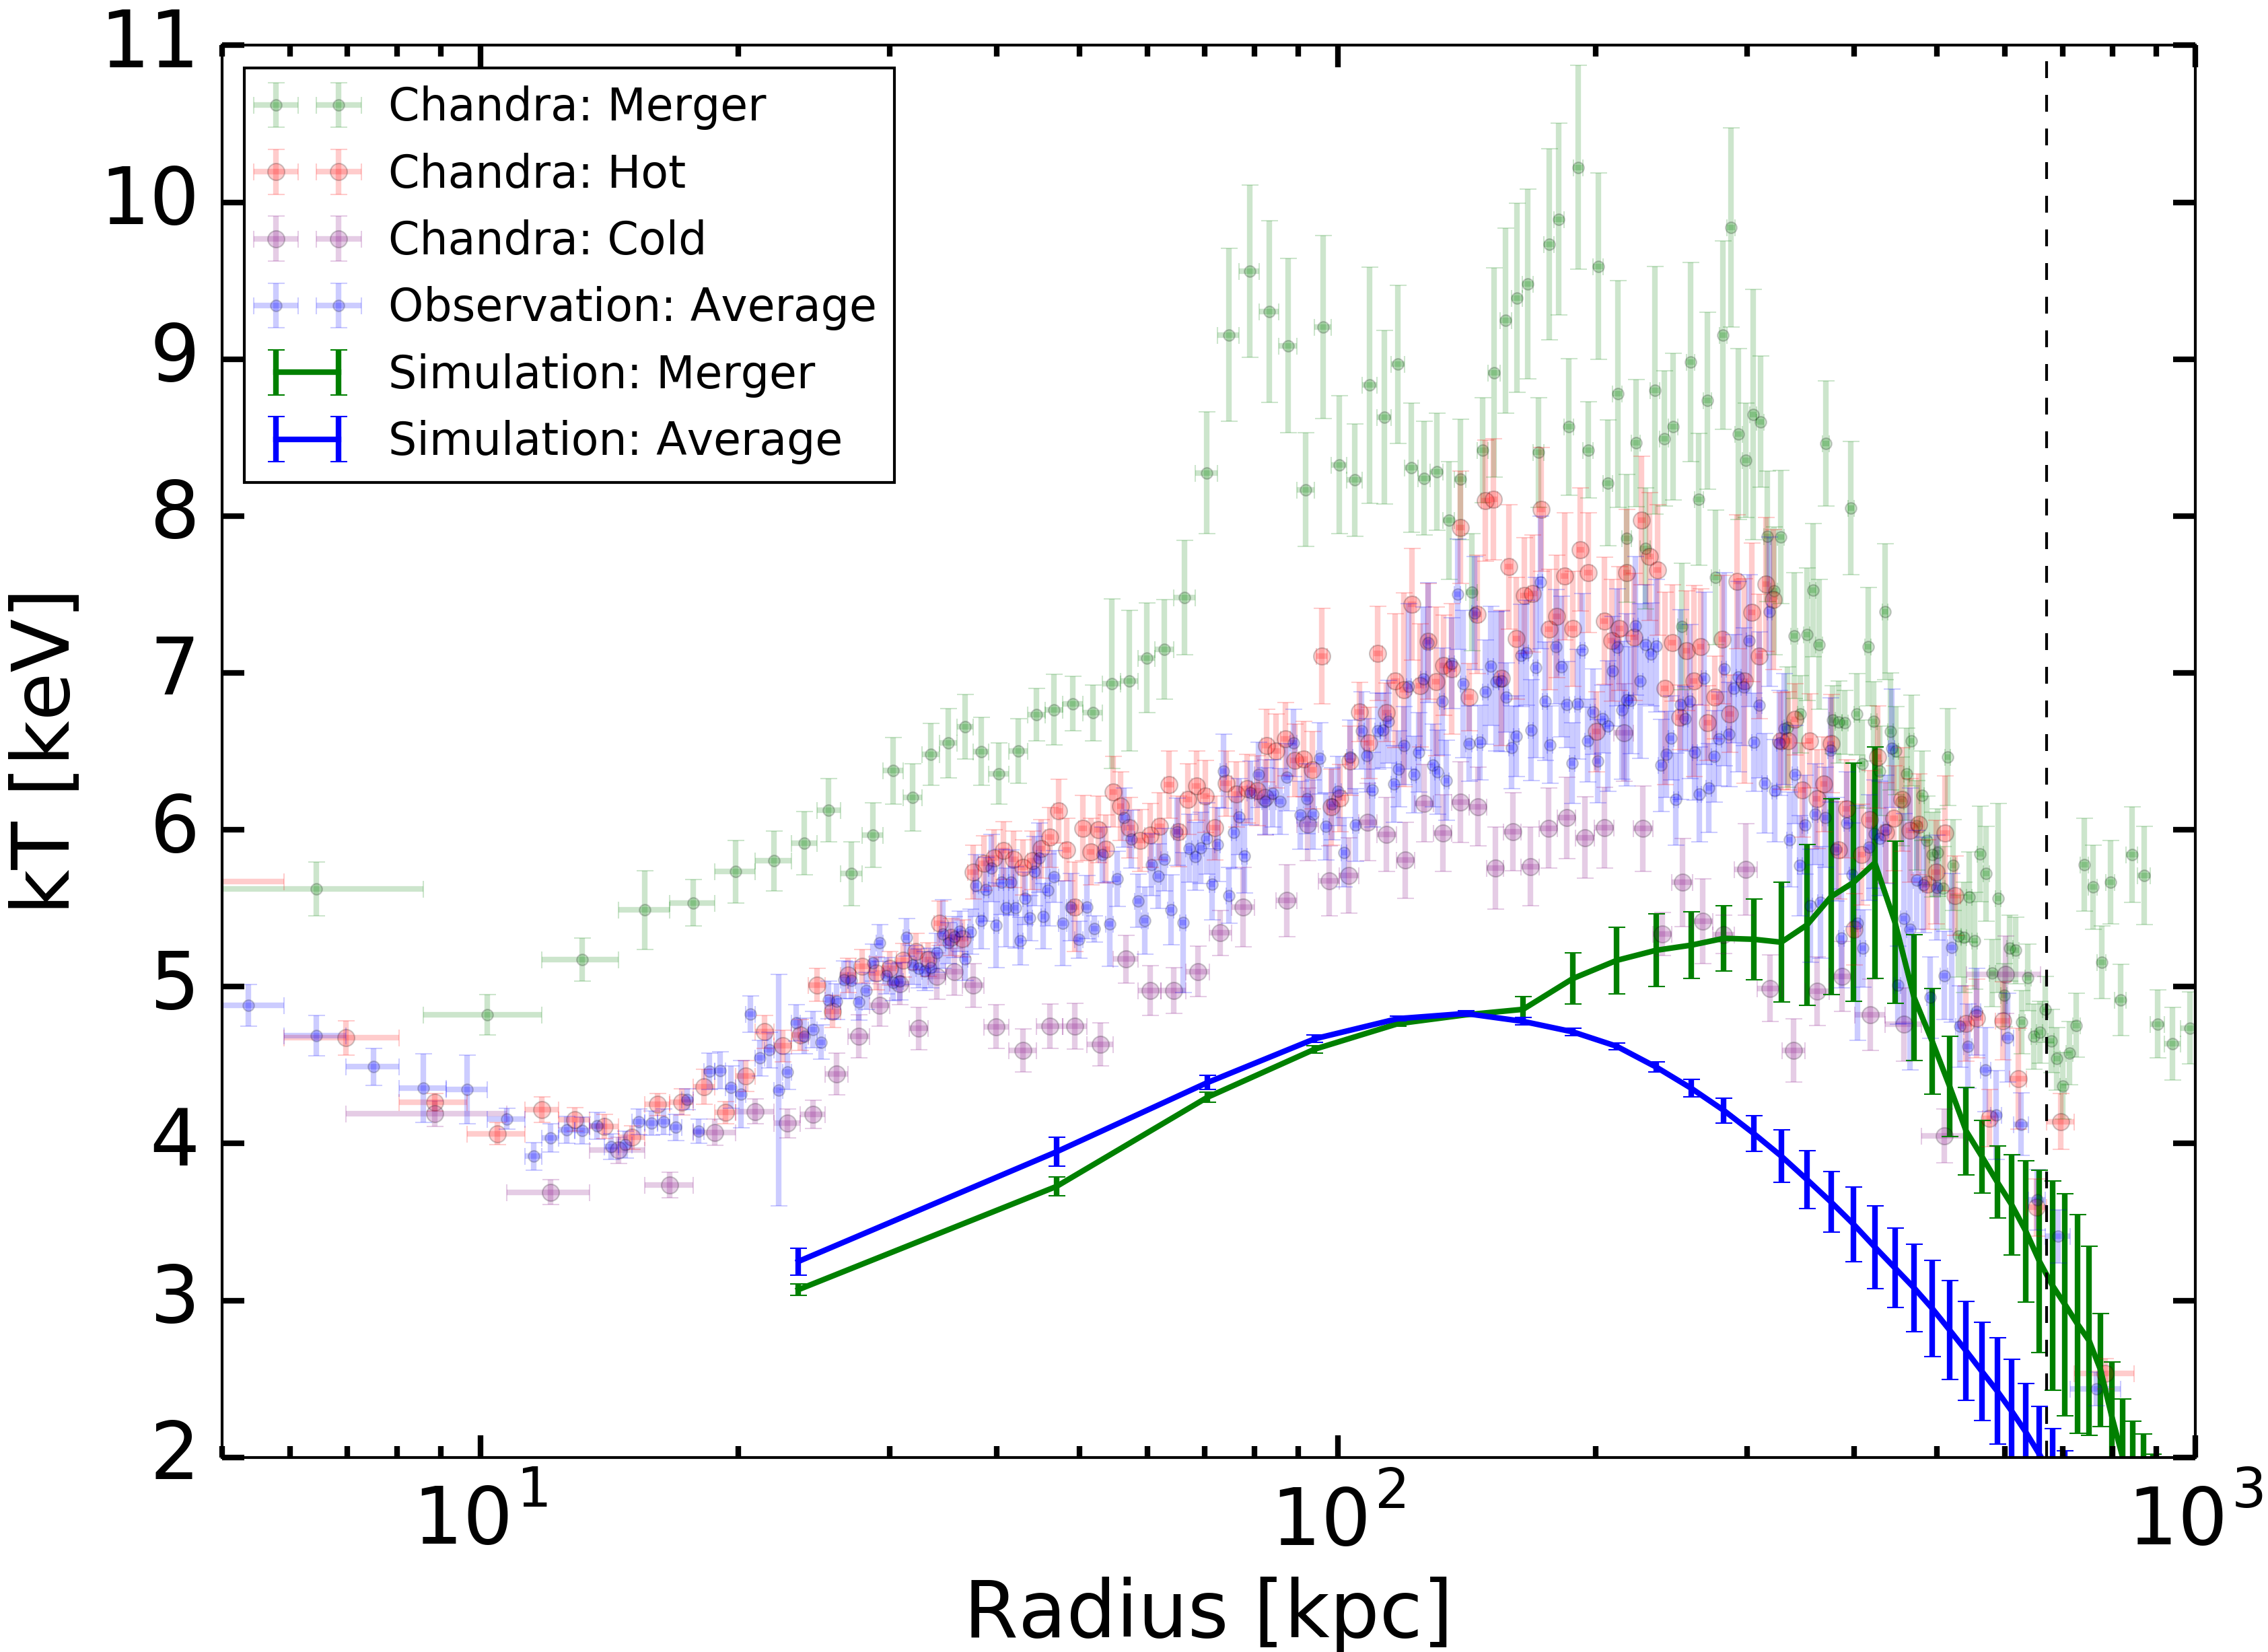
\includegraphics[width=0.85\textwidth]{sim/temperature/20160820T0403_temperature.png}
    \caption{Spectroscopic temperature of the $\epsilon = 0.8$ simulation.}
    \label{fig:20160820T0403_T}
\end{figure}
\clearpage

\begin{figure}
    \centering
    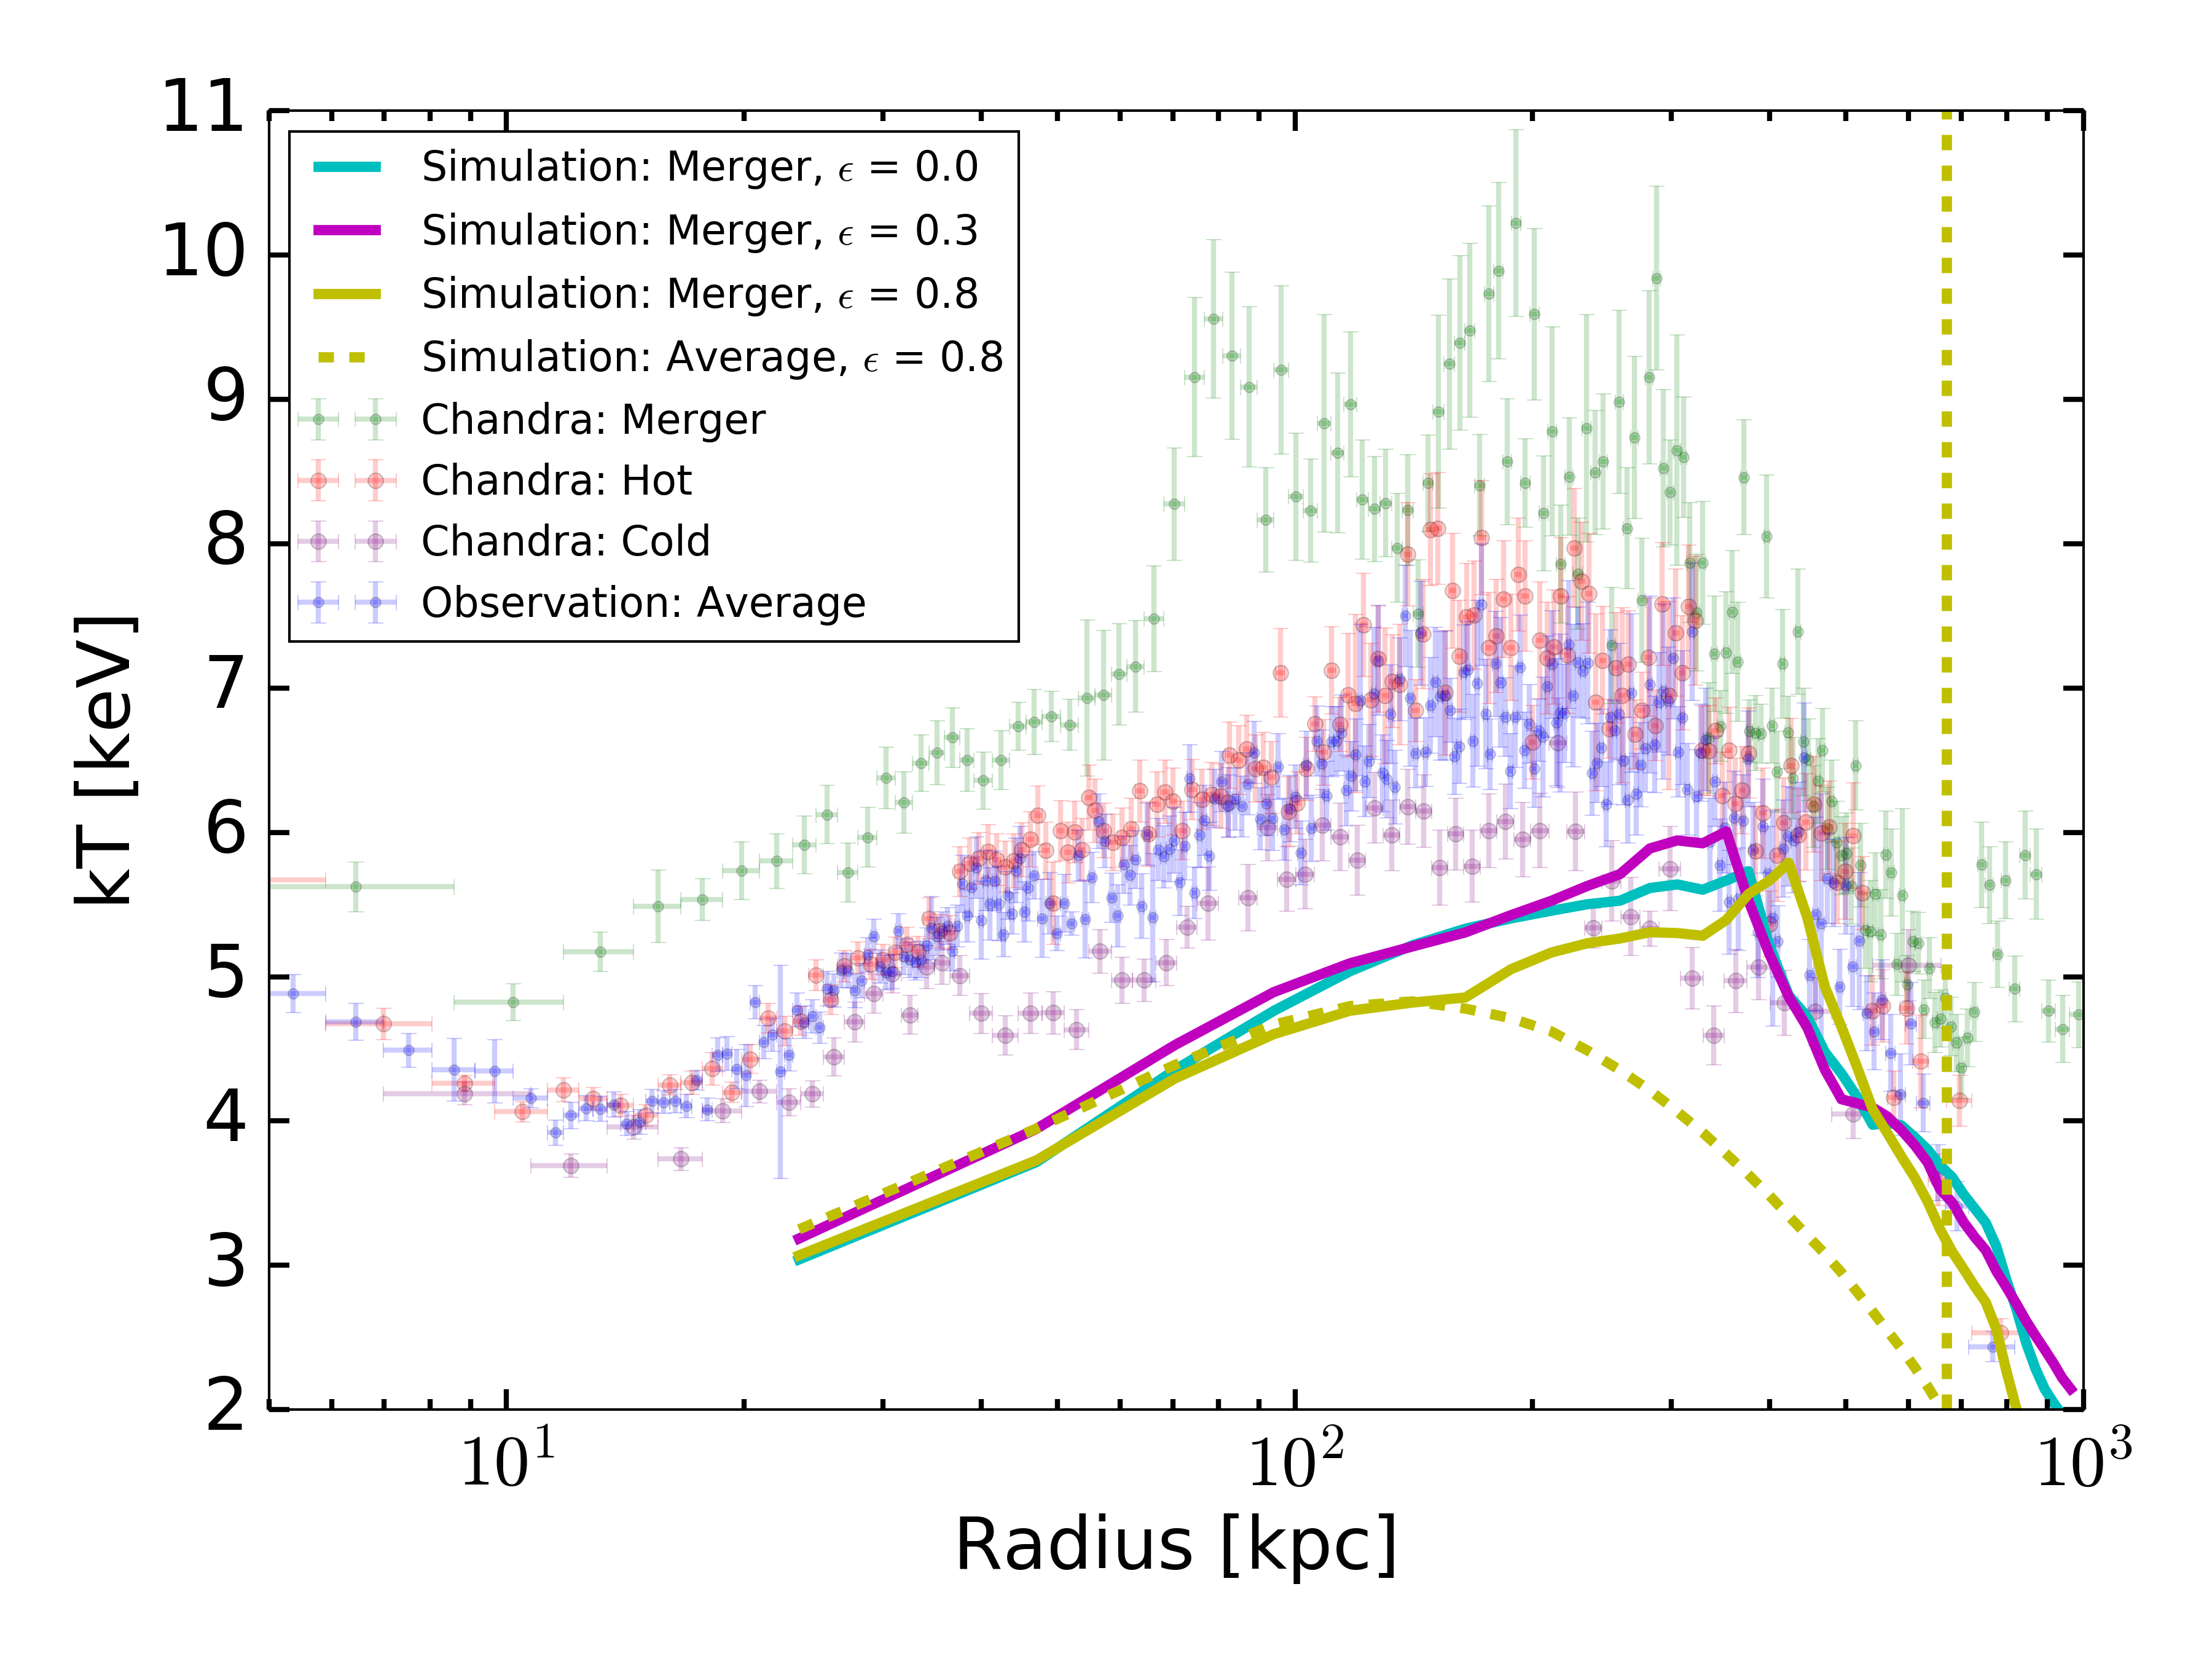
\includegraphics[width=\textwidth]{sim/temperature/temperature_comparison.png}
    \caption{Spectroscopic temperature of the $\epsilon \in [0.0, 0.3, 0.8]$ 
             simulations indicate that the induced temperature jump is not
             influenced significantly by the initial (and merger) velocity. Only
             the average profile of the third model is shown as the quiescent 
             temperature profiles are very similar. The dashed vertical line
             indicates the location of CygB in the same simulation run.}
    \label{fig:tjump_vs_velocity}
\end{figure}

We now turn to the \satellite{Suzaku} observations to investigate consistency
between the simulated and the \satellite{Chandra} observed temperature profiles.
The \satellite{Suzaku} data is included in Figure~\ref{fig:TimesFourOverThree}, and
Figure~\ref{fig:MergerversusSuzakuObservation} shows the simulated temperature 
profiles without artificial increasing the temperature versus the \satellite{Suzaku}observation. The latter data is obtained by eye from \citet{2013AN....334..346S},
where the values on the x-axis in the conference proceeding span a range from
$-2$ up to $12.3$ in units of arcminute which is converted to kpc. In this 
comparison we also see that the simulated temperature profile is significantly
lower than the \satellite{Suzaku} observation. Neither adding a factor $1.5$~keV 
nor multiplying by $4/3$ would give a consistent picture. Furthermore, we note
that the \satellite{Suzaku} and \satellite{Chandra} observations at larger radii 
seem to be inconsistent within the error bars. However, we do not know
the method used to extract the \satellite{Suzaku} spectrum and therefore we
cannot interpret these differences. We could speculate that a rectangular box 
could be used by \citet{2013AN....334..346S}. Therefore we show the temperature 
structure when using the ds9 \mybox{Region} $\rightarrow$ \mybox{Shape} 
$\rightarrow$ \mybox{Projection} tool to create such a boxed region. The extraction
regions are indicated in Figure~\ref{fig:BoxExtraction}, and the resulting 
temperature profiles are given in Figure~\ref{fig:BoxExtractionT}. We note that
the average profiles seem consistent (blue solid and blue dashed line), but that
the temperature shows a double peak within the box region and that for the same
initial velocity a higher temperature jump is observed this way.

% \begin{figure}
%     \centering
%     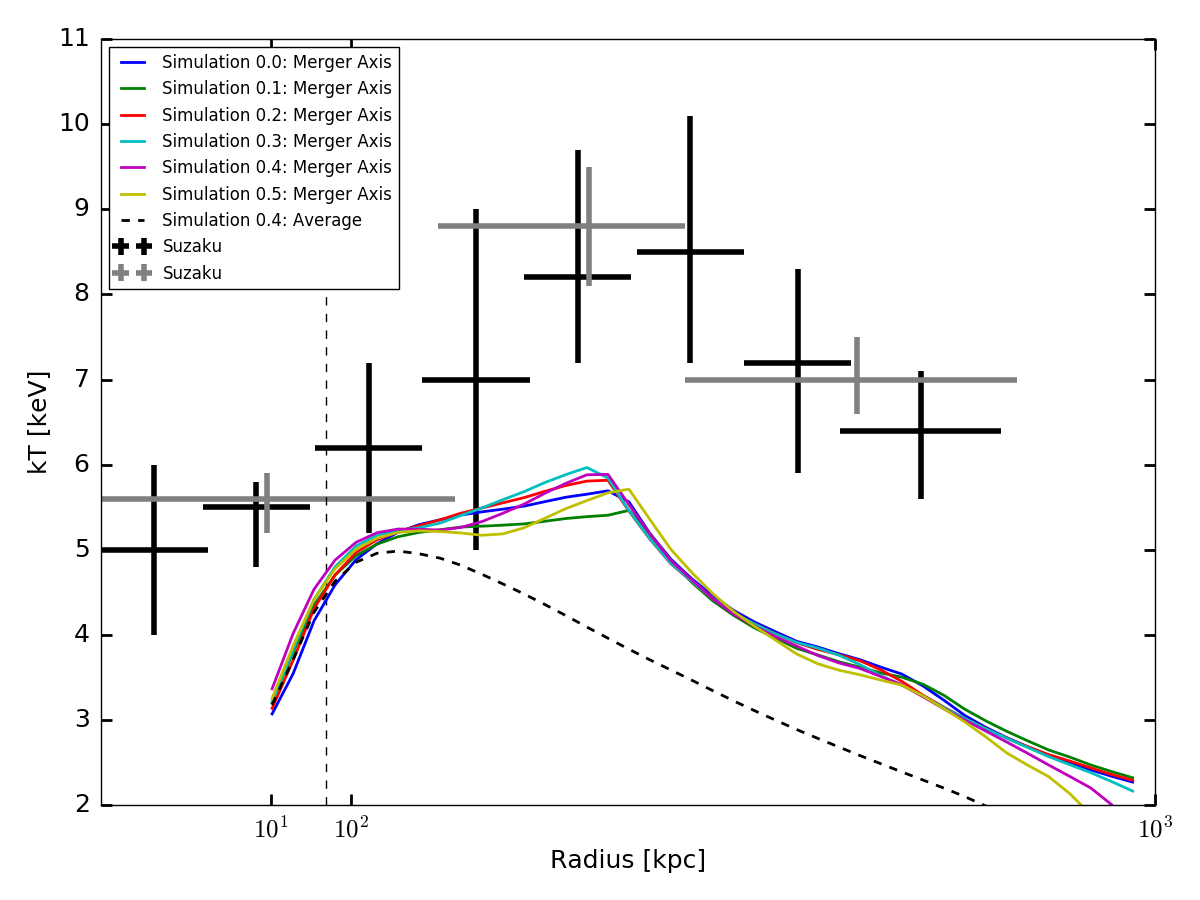
\includegraphics[width=0.9\textwidth]{sim/temperature/SimulationVersusSuzaku.png}
%     \caption{Simulation versus observation, where the $270^\circ$ non-merger wedge
%              is used as average, hydrostatic temperature structure. 
%          }
%     \label{fig:MergerversusSuzakuObservation}
% \end{figure}

\newpage

We consider several possible interpretations of these results. Firstly, we examine
a geometry-related cause of the discrepancy between the simulation and the 
observation. Secondly, we consider that the hydrostatic temperature structure 
(which is simulated) is significantly lower than the observed temperature, 
which could be a sign of a significant amount of heating the cluster gas (up
to one mega parsec) by the central AGN in the Cygnus~A galaxy. Finally, we consider
the possibility that the simulation shows the correct temperature structure, 
although the overall temperature structure for some reason is too low. The latter 
would imply mistakes were made along the way in the simulation or in the analysis
performed on the simulated emission weighted temperature.




\subsection{Varying the projection angle}
\label{sec:ProjectionAngle}



\SubfileBibliography
\end{document}
